\documentclass[
11pt, % Set the default font size, options include: 8pt, 9pt, 10pt, 11pt, 12pt, 14pt, 17pt, 20pt
%t, % Uncomment to vertically align all slide content to the top of the slide, rather than the default centered
%aspectratio=169, % Uncomment to set the aspect ratio to a 16:9 ratio which matches the aspect ratio of 1080p and 4K screens and projectors
]{beamer}

\graphicspath{{Images/}{./}} % Specifies where to look for included images (trailing slash required)

\usepackage{todonotes}
\usepackage{graphicx}
\usepackage{xcolor}
\usepackage{subfig}
%%\usepackage[noend]{algpseudocode}

%
%\usepackage{algorithm}
%\usepackage{algorithmic}
\usepackage{algorithm}
\usepackage{algpseudocode}
\usepackage{blkarray}
\usepackage{amsmath}
\usepackage{xspace}
\usepackage{float}


\usepackage{tikz}
\usetikzlibrary{matrix, decorations, patterns, positioning, shapes, calc, intersections, arrows, fit}

\usetikzlibrary{patterns}
\usetikzlibrary{fit,calc,positioning,decorations.pathreplacing,matrix,3d, hobby}

\usepackage{booktabs} % Allows the use of \toprule, \midrule and \bottomrule for better rules in tables
\usepackage{bm}

\newcommand{\brown}[1]{{\color{brown} #1 }}

%% Colors from https://latexcolor.com/
\definecolor{pastelviolet}{rgb}{0.8, 0.6, 0.79}
\definecolor{babyblueeyes}{rgb}{0.63, 0.79, 0.95}
\definecolor{pastelyellow}{rgb}{0.99, 0.99, 0.59}
\definecolor{pastelgreen}{rgb}{0.47, 0.87, 0.47}
\definecolor{pastelred}{rgb}{1.0, 0.41, 0.38}
\colorlet{patternblue}{blue!60}


\colorlet{darkred}{red!80!black}
\colorlet{darkblue}{blue!80!black}
\newcommand<>{\darkred}[1]{{\color{darkred}{#1}}}
\newcommand<>{\darkblue}[1]{{\color#2{blue!50!black!100}{#1}}}

\newcommand{\A}{\mathbf{A}}
\newcommand{\B}{\mathbf{B}}
\newcommand{\CC}{\mathbf{C}}
\newcommand{\Real}{\mathbb{R}}
\newcommand{\vc}[1]{\bm{#1}}

\usetheme{Madrid}

%\usepackage{enumitem}



%----------------------------------------------------------------------------------------
%	PRESENTATION INFORMATION
%----------------------------------------------------------------------------------------

\title[Matrix factorization]{Matrix factorization} % The short title in the optional parameter appears at the bottom of every slide, the full title in the main parameter is only on the title page

%\subtitle{Optional Subtitle} % Presentation subtitle, remove this command if a subtitle isn't required

\author[Suraj Kumar]{Suraj Kumar} % Presenter name(s), the optional parameter can contain a shortened version to appear on the bottom of every slide, while the main parameter will appear on the title slide

\institute[Inria \& ENS Lyon]{Inria \& ENS Lyon \\ \smallskip Email:\textit{suraj.kumar@inria.fr}} % Your institution, the optional parameter can be used for the institution shorthand and will appear on the bottom of every slide after author names, while the required parameter is used on the title slide and can include your email address or additional information on separate lines

\date[CR12]{CR12: September 2023\\ \smallskip\small https://surakuma.github.io/courses/daamtc.html} % Presentation date or conference/meeting name, the optional parameter can contain a shortened version to appear on the bottom of every slide, while the required parameter value is output to the title slide

%----------------------------------------------------------------------------------------

\begin{document}
	
	%----------------------------------------------------------------------------------------
	%	TITLE SLIDE
	%----------------------------------------------------------------------------------------
	
	\begin{frame}
		\titlepage % Output the title slide, automatically created using the text entered in the PRESENTATION INFORMATION block above
	\end{frame}
	\begin{frame}{Matrix factorizations}
		\begin{itemize}
			\item Useful to solve systems of linear equations $Ax=b$
			\item Popular factorizations
			\begin{itemize}
				\item LU factorization
				\item QR factorization
				\item Cholesky factorization
				\item Singular Value Decomposition (SVD)
			\end{itemize}
		\end{itemize}
	\end{frame}

	\begin{frame}{Important norm definitions }
		\begin{block}{Vector norm for $x\in \mathbb{R}^n$}
%			Given a $x\in \mathbb{R}^n$, 
%			n-dimension vector $\mathbf{x}=\begin{pmatrix}
%			x_1\\
%			x_2\\
%			\vdots\\
%			x_n
%			\end{pmatrix}$,
			The Euclidean norm of $x$ is represented as $||\mathbf{x}||$ or $||\mathbf{x}||_2$ and defined as 
			$||\mathbf{x}|| = \sqrt{\sum_{i=1}^{n}x_i^2}$
		\end{block}
	\vfill
	\begin{block}{Matrix norm for $A\in \mathbb{R}^{n\times n}$}
		\begin{itemize}
			\item[] $$\textnormal{Frobenius norm, } ||A||_F = \sqrt{\sum_{j=1}^{n}\sum_{i=1}^{n}{A_{ij}}^2} = \sqrt{trace(AA^T)}$$
			\item[] $$\textnormal{Spectral norm, }||A||_2 = \textnormal{largest singular value of A}$$
		\end{itemize}
	\end{block}
	\end{frame}
	\section{LU factorization}
	\begin{frame}{Table of Contents}		
		\tableofcontents[currentsection,hideallsubsections] % Output the table of contents (all sections on one slide)		
	\end{frame}

\begin{frame}{Algebra of LU factorization with an example}
	Given the matrix $A = \begin{pmatrix}
	2 & 6 & 5\\
	4 & 15 & 11\\
	6 & 30 & 23
	\end{pmatrix}$
	\vfill
	\begin{itemize}
		\item Let $L_1 = \begin{pmatrix}
		1 & 0 & 0\\
		-2 & 1 & 0\\
		-3 & 0 & 1\\
		\end{pmatrix} $, $L_1A=\begin{pmatrix}
		2 & 6 & 5\\
		0 & 3 & 1\\
		0 & 12 & 8		
		\end{pmatrix}$
		\vfill
		\item Let $L_2=\begin{pmatrix}
		 1 & 0 & 0\\
		 0 & 1 & 0 \\
		 0 & -4 & 1
		\end{pmatrix}$, $L_2L_1A=\begin{pmatrix}
		2 & 6 & 5\\
		0 & 3 & 1\\
		0 & 0 & 4
		\end{pmatrix}$
		\vfill
		\item Let $U=\begin{pmatrix}
		2 & 6 & 5\\
		0 & 3 & 1\\
		0 & 0 & 4
		\end{pmatrix}$, $L_2L_1A=U$
	\end{itemize}
\end{frame}
\begin{frame}{Algebra of LU factorization}
	
	{\small
		
	$L_2L_1A=U \implies A= (L_2L_1)^{-1}U = L_1^{-1}L_2^{-1}U$
	\vfill
	 $L_1$=$\begin{pmatrix}
	1 & 0 & 0\\
	-2 & 1 & 0\\
	-3 & 0 & 1\\
	\end{pmatrix} $, $L_1^{-1}$=$\begin{pmatrix}
	1 & 0 & 0\\
	2 & 1 & 0\\
	3 & 0 & 1\\
	\end{pmatrix}$, $L_2$=$\begin{pmatrix}
	1 & 0 & 0\\
	0 & 1 & 0 \\
	0 & -4 & 1
	\end{pmatrix}$, $L_2^{-1}$=$\begin{pmatrix}
	1 & 0 & 0\\
	0 & 1 & 0 \\
	0 & 4 & 1
	\end{pmatrix}$
	\vfill 
	$\qquad\qquad\qquad\qquad\qquad\qquad L_1^{-1}L_2^{-1} = \begin{pmatrix}
	1 & 0 & 0\\
	2 & 1 & 0\\
	3 & 4 & 1\\
	\end{pmatrix}$
	\vfill 

	$A=\begin{pmatrix}
			2 & 6 & 5\\
			4 & 15 & 11\\
			6 & 30 & 23
		\end{pmatrix} = \begin{pmatrix}
		1 & 0 & 0\\
		2 & 1 & 0\\
		3 & 4 & 1\\
		\end{pmatrix}\begin{pmatrix}
		2 & 6 & 5\\
		0 & 3 & 1\\
		0 & 0 & 4
		\end{pmatrix} = LU$, where $L=L_1^{-1}L_2^{-1}$
}
\end{frame}
	\begin{frame}{The need of pivoting  (or row exchanges): $PA=LU$}
	\begin{itemize}
		\item To avoid division by $0$ or small diagonal elements (for stability)
		\item $A= \begin{pmatrix}
		0 & 2 & 4\\
		3 & 1 & 2\\
		6 & 8 & 7
		\end{pmatrix}$ has an LU factorization if we permute the rows of the matrix $A$
		$$PA=\begin{pmatrix}
		3 & 1 & 2\\
		0 & 2 & 4\\
		6 & 8 & 7
		\end{pmatrix} = \begin{pmatrix}
		1 & 0 & 0\\
		0 & 1 & 0\\
		2 & 3 & 1\\
		\end{pmatrix} 
		\begin{pmatrix}
		3 & 1 & 2\\
		0 & 2 & 4\\
		0 & 0 & -9
		\end{pmatrix}$$
		
		$\qquad\qquad\qquad$Here $P=\begin{pmatrix}
		0 & 1 & 0\\
		1 & 0 & 0\\
		0 & 0 & 1
		\end{pmatrix}$			 
	\end{itemize}
\end{frame}







	\begin{frame}{Communication lower bounds}
		\begin{itemize}
%			\item People obtain results for matrix multiplication operations
			\item Matrix multiplication lower bounds apply to LU factorization using reduction [Ballard et. al., 09]
%			, for instance, bound for LU factorization\vspace*{-0.15cm}
			{\scriptsize\begin{align*}
				\begin{pmatrix}
				I &  & -B\\
				A & I &  &\\
				& & I
				\end{pmatrix}
				&=
				\begin{pmatrix}
				I & &\\
				A & I & \\
				&& I
				\end{pmatrix}
				\begin{pmatrix}
				I & & -B \\
				& I & AB\\
				& & I
				\end{pmatrix}
				\end{align*}}
		\end{itemize}
%	\vfill
	\begin{block}{Lower bounds}
	\begin{itemize}
		\item Sequential lower bound on bandwidth = $\Omega(\frac{n^3}{\sqrt{M}})$
		\vfill
		\item Memory-dependent parallel lower bound on bandwidth = $\Omega(\frac{n^3}{P\sqrt{M}})$
		\vfill
		\item Memory-independent parallel lower bound on bandwidth = $\Omega\left(\frac{n^3}{P^\frac23}\right)$
	\end{itemize}
	\end{block}
	\end{frame}

	\begin{frame}
	\frametitle{LU Factorization (1/2)}
	\begin{minipage}{0.65\linewidth}
		LU factorization (Gaussian elimination):
		\begin{itemize}
			\item Convert a matrix $A$ into product $L\times U$
			\item $L$ is lower triangular with diagonal 1
			\item $U$ is upper triangular
			\item $L$ and $U$ stored in place with $A$
		\end{itemize}
	\end{minipage}~~~
	\begin{minipage}{0.3\linewidth}
		\includegraphics[width=\linewidth]{lu-final.pdf}
	\end{minipage}
	\vfill
	\begin{block}{LU Algorithm}
		For $k=1\ldots n-1$:
		\begin{itemize}
			\item For $i=k+1\ldots n$, \\
			$A_{i,k} \gets A_{i,k}/A_{k,k}$ (column/panel preparation)
			\item For $i=k+1\ldots n$, \\
			~~For $j=k+1\ldots n$, \\
			~~~~$A_{i,j} \gets A_{i,j} - A_{i,k} A_{k,j}$ (update)
		\end{itemize}
	\end{block}
\end{frame}
\begin{frame}{Block LU factorization}
	\begin{block}{Partition of a $n \times n$ matrix $A$}
		$$A=\begin{pmatrix}
		A_{11} & A_{12}\\
		A_{21} & A_{22}
		\end{pmatrix}$$
	Here $A_{11}$ is of size $b \times b$, $A_{21}$ is of size $(n-b) \times b$, $A_{12}$ is of size $b \times (n-b)$ and $A_{22}$ is of size $(n-b) \times (n-b)$. 
	\end{block}
	\vfill
	\begin{block}{Structure of LU factorization algorithm}
		\begin{itemize}
			\item The first iteration computes the factorization:
			$$A=\begin{pmatrix}
			A_{11} & A_{12}\\
			A_{21} & A_{22}
			\end{pmatrix} = \begin{pmatrix}
			L_{11} & \\
			L_{21} & I_{n-b}
			\end{pmatrix}
			\begin{pmatrix}
			U_{11} & U_{12}\\
			& A'
			\end{pmatrix}$$
			\item The algorithm continues recursively on the trailing matrix $A'$.
		\end{itemize}
	\end{block}
\end{frame}
\begin{frame}{Block LU factorization}
	\begin{enumerate}
		\item Compute the LU factorization of the first block column
		$$\begin{pmatrix}
		A_{11}\\
		A_{21}
		\end{pmatrix} = \begin{pmatrix}
		L_{11}\\
		L_{21}
		\end{pmatrix}U_{11}$$
		\vfill
		\item Solve the triangular system 
		$$L_{11}U_{12}= A_{12}$$
		\vfill
		\item Update the trailing matrix
		$$A' = A_{22}- L_{21}U_{12}$$
		\vfill
		\item Compute recursively the block LU factorization of $A'$
	\end{enumerate}
\end{frame}
	\section{QR factorization}
	
	\begin{frame}{Terminology related to QR factorization}
		
		\small
		
		An \textbf{orthogonal} matrix $Q$ satisfies $Q^TQ=QQ^T=I$ (the identity matrix)
		\begin{itemize}
			\item $Q$ must be square
			\item $Q$'s rows are orthogonal to each other and have unit norm
			\item $Q$'s columns are orthogonal to each other and have unit norm
		\end{itemize}
		
		\vfill \pause
		
		A matrix $U$ has \textbf{orthonormal columns} if $U^TU=I$ (the identity matrix)
		\begin{itemize}
			\item $U$'s columns are orthogonal to each other and have unit norm
			\item $U$ can have more rows than columns, in which case $UU^T\neq I$
		\end{itemize}
		
		\vfill \pause
		
		Given a matrix $A$, we can \textbf{orthogonalize} its columns by finding a matrix $Q$ such that
		\begin{itemize}
			\item $Q$'s columns span the same space as $A$'s columns
			\item $Q$ has orthonormal columns
			\item there exists a nonsingular matrix $Z$ such that $A=QZ$
		\end{itemize}
		
	\end{frame}
	
	
	\begin{frame}{QR factorization}
		
		The \textbf{QR factorization} is a fundamental matrix factorization:
		$$A = QR = \begin{bmatrix} \hat{Q} & \tilde{Q} \end{bmatrix} \begin{bmatrix} \hat{R} \\ 0 \end{bmatrix} = \hat{Q} \hat{R}$$
		\begin{itemize}
			\item if $A$ is $m\times n$, $m\geq n$, then $Q$ is $m\times m$, $R$ is $m\times n$, $\hat{Q}$ is $m\times n$, and $\hat{R}$ is $n\times n$
			\item $Q$ is orthogonal, $\hat{Q}$ has orthonormal columns, and $R$ is upper triangular
			\item $\hat{Q}$ is an orthogonalization of $A$
		\end{itemize}
		
	\end{frame}
	\begin{frame}
		\frametitle{Classical algorithms for QR factorization}
		
		\begin{enumerate}
			\item Gram-Schmidt process
			\begin{itemize}
				\item intuitive: each vector is orthogonalized against previous ones by subtracting out components of the vector in previous directions
				\item has numerical problems (vectors aren't always numerically orthonormal)
				\item two variants ``classical'' and ``modified'' are mathematically identical
			\end{itemize}
			\vfill
			\item Householder QR
			\begin{itemize}
				\item uses orthogonal matrices to transform input to triangular form
				\item numerically stable
			\end{itemize}
%			\vfill
%			\item Cholesky QR
%			\begin{itemize}
%				\item simplest and cheapest algorithm
%				\item has numerical problems (vectors aren't always numerically orthonormal)
%			\end{itemize}
		\end{enumerate}
		
	\end{frame}
	\begin{frame}
		\frametitle{Gram-Schmidt}
		
		\textcolor{blue}{
			\only<1>{Classical Gram-Schmidt (CGS) process}
			\only<2>{Modified Gram-Schmidt (MGS) process}
		}
		
		\begin{algorithmic}
			\Require $A = \begin{bmatrix} x_1 & x_2 & \cdots & x_n \end{bmatrix}$
			\For{$i=1$ to $n$}
			\State $v_i = x_i$
			\For{$j=1$ to $i-1$}
			\State $r_{ji} = q_j^T\textcolor{red}{\only<1>{x_i}\only<2>{v_i}}$ \Comment{compute size of projection of \textcolor{red}{\only<1>{$i$th col of $A$}\only<2>{current vector}} onto $q_j$}
			\State $v_i = v_i - r_{ji} q_j$ \Comment{remove this component from vector $v_i$}
			\EndFor
			\State $r_{ii}=\|v_i\|_2$
			\State $q_i = v_i/r_{ii}$ \Comment{normalize vector}
			\EndFor
			\Ensure $Q = \begin{bmatrix} q_1 & q_2 & \cdots & q_n \end{bmatrix}$ has orthonormal columns
			\Ensure $R$ is upper triangular and $A=QR$
		\end{algorithmic}
	\end{frame}

	\begin{frame}{Householder transformation}
		\begin{minipage}{0.57\linewidth}
			
			\begin{itemize}
				\item $v$ is a unit vector
				\vfill
				\item The reflection hyperplane can be defined by its normal vector $v$
				\vfill
				\item $(I-2vv^T)x$ is the reflection of point $x$ with the hyperplane 
			\end{itemize}
		\end{minipage}
	\begin{minipage}{0.4\linewidth}

				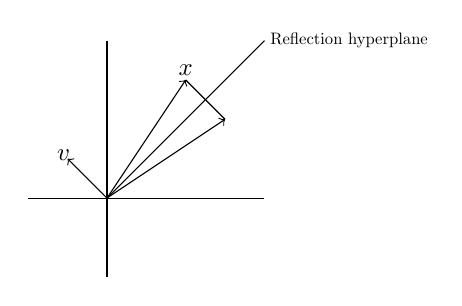
\begin{tikzpicture}[scale=0.5, every node/.style={transform shape}]
				
				\draw (0,-2) -- (0,4);
				\draw (-2,0) -- (4,0);
				\draw (0,0) -- (4,4);
				
				\draw [->] (0,0) -- (3,2);
				\draw [->] (0,0) -- (2,3);
				\draw  (3,2) -- (2,3);
				
				\draw [->] (0,0) -- (-1,1);
				
				\node [scale=1.8] at (-1.1,1.1) {$v$};
				\node [scale=1.8] at (2,3.25) {$x$};
				\node [scale=1.2,right] at (4,4) {Reflection hyperplane};
		\end{tikzpicture}
	\end{minipage}
\vfill
	\begin{itemize}
		\item $P=I-2vv^T$ matrix is known as the Householder matrix
		\vfill
		\item $P$ is symmetric and orthogonal, $P^2=I$
	\end{itemize}
	\end{frame}

\begin{frame}{Main idea of Householder QR factorization}
%	\begin{itemize}
%		\item[] 
		Look for a Householder matrix that annihilates the elements of a vector $x$, except first one:	
		$$Px=y, ||x||_2=||y||_2, y=\sigma e_1, \sigma=\pm ||x||_2$$
		
		\vfill
		
		The choice of sign is made to avoid cancellation or small numerical values while computing $v_1=x_1-\sigma$. Here $v_1$, $x_1$ are the first elements of vectors $v$, $x$ respectively. 
		
		$$v=x-y=x-\sigma e_1$$
		$$\qquad\qquad\sigma=-sign(x1)||x||_2, v=x-\sigma e_1$$
		$$\qquad u=\frac{v}{||v||_2}, P=I-2 uu^T$$
%	\end{itemize}

\end{frame}
\begin{frame}{Householder QR algorithm}
	
	Given vector $x$, a \textbf{Householder transformation} $I-2uu^T$ maps $x$ to $\sigma e_1$
	\begin{itemize}
		\item $u$ is called the \textbf{Householder vector}
%		\item a Householder transformation is an orthogonal matrix
	\end{itemize}
	
	\vfill
	
	\begin{algorithmic}
		\Require $A = \begin{bmatrix} x_1 & x_2 & \cdots & x_n \end{bmatrix}$
		\For{$i=1$ to $n$}
		\State Compute Householder vector $u_i$ from $x_i$
		\State $A = (I-2u_iu_i^T)A$ \Comment{apply Householder transformation}
%		= A - (2u_i)(u_i^TA)$ 
		\EndFor
		\State $R=A$
		\Ensure $U = \begin{bmatrix} u_1 & u_2 & \cdots & u_n \end{bmatrix}$ is lower triangular
		\Ensure $R$ is upper triangular and $A=(I-2u_1u_1^T)\cdots(I-2u_nu_n^T)R$
	\end{algorithmic}
	
\end{frame}

	\section{SVD}

%	\section{Popular data layouts}
%\begin{frame}{Table of Contents}		
%	\tableofcontents[currentsection,hideallsubsections] % Output the table of contents (all sections on one slide)		
%\end{frame}

\end{document} 